\section{Introduction}
\label{sec:introduction}
\PARstart{A}{utonomous} ground robots are increasingly used to inspect
electrical substations, where regular checks of transformers, breakers and
busbars are essential but expose human operators to high-voltage
hazards~\cite{li2024state}. A typical inspection robot follows a
planned round between points of interest and runs a perception pipeline to read
meters, recognize switch states and measure temperatures, and recent work has
improved the routing itself with learning-based
planners~\cite{zhang2025substation}.

\begin{figure}[t]
\centering
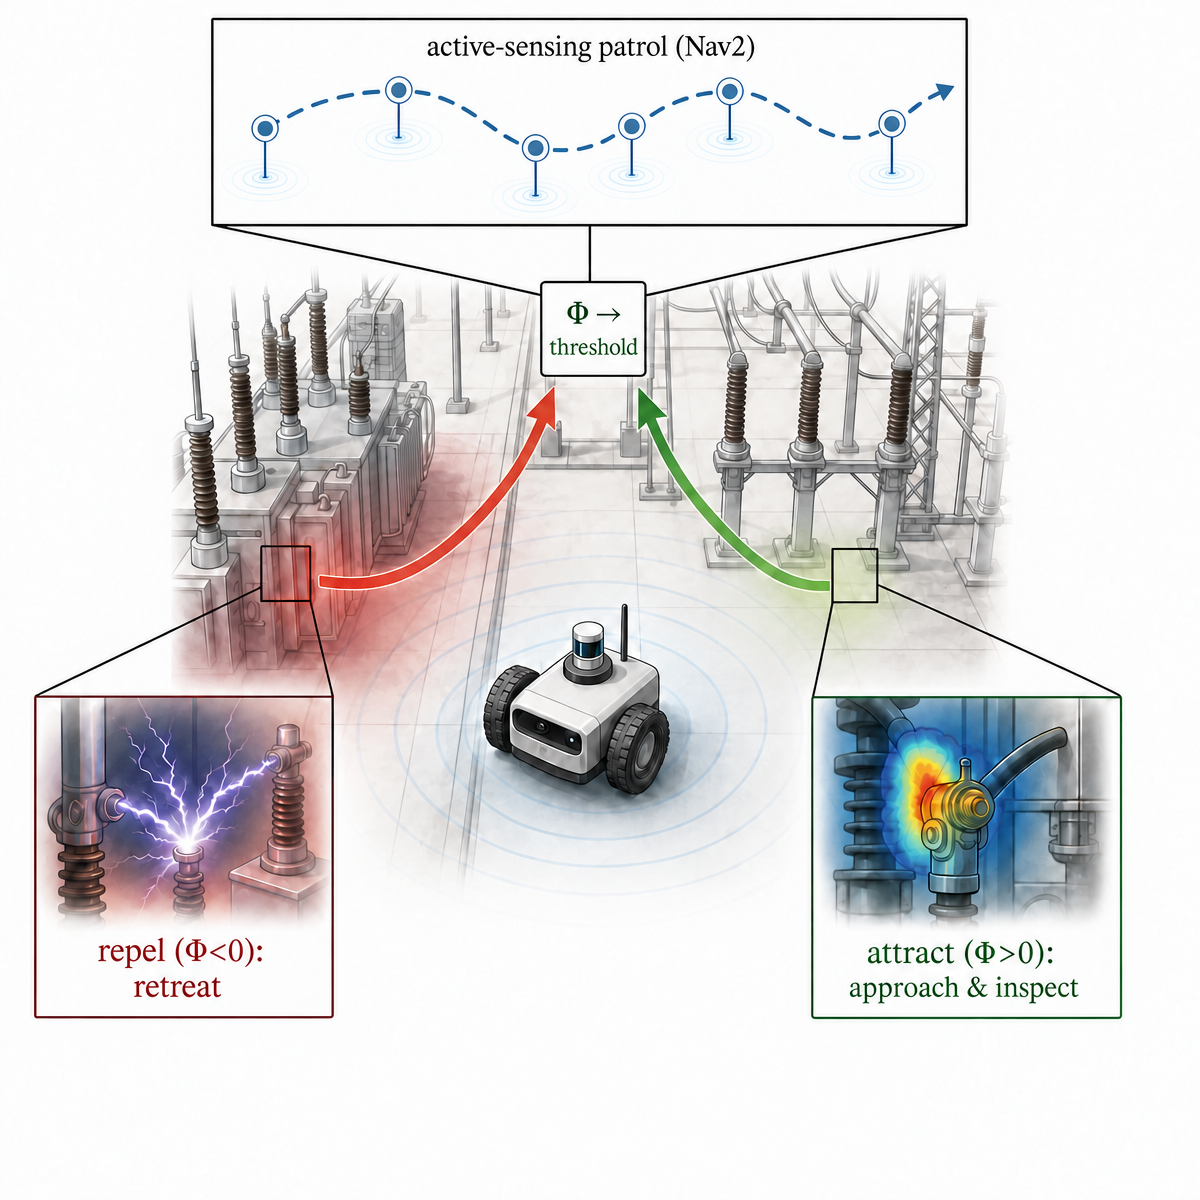
\includegraphics[width=\columnwidth]{concept_overview}
\caption{Concept overview. A deliberative \emph{active-sensing} patrol (Nav2)
carries the robot around the substation, while a \emph{reactive}
layer makes it approach anomalies (attraction) and retreat from hazards
(repulsion) via a threshold on the raw saliency field $\bm{\Phi}$. The same field is
also expressible as an additive term in a tabular value update, recorded as a
design note in Appendix~\ref{app:update} because it does not drive the executed
behavior.}
\label{fig:concept}
\end{figure}

Yet most deployments treat the round as a \emph{fixed coverage} problem: the
robot drives between waypoints and classifies whatever appears, without
adapting its motion to what it senses. The complementary failure mode is the
\emph{purely reactive} controller, which responds only to stimuli already
within sensor range and, in the absence of a stimulus, has nothing to act
upon---besides being prone to local-minima stalls~\cite{koren1991}. What is
missing is a mechanism that (i) carries the sensors to where relevant events may
occur and (ii), once an event is within range, reacts to it---approaching an
anomaly to inspect it, or retreating from a danger.

Our key observation is that these two needs map onto two layers
(Fig.~\ref{fig:concept}). Bringing the
sensors to potential events is a form of \emph{active
sensing}~\cite{bajcsy1988}: the inspection round itself performs this
placement. Reacting to a sensed event is an \emph{affective}
impulse~\cite{breazeal2003}: an attraction toward salient anomalies or a
repulsion from hazards. We realize the second layer as a
threshold-triggered controller driven by a field $\Phi(s)$---positive for
attraction, negative for repulsion, derived from sensory saliency---whose sign
carries a categorical safety precedence. We run this reactive layer on top of a
standard deliberative stack (Nav2 with a Model Predictive Path Integral (MPPI)
controller~\cite{macenski2020nav2,williams2017mppi}), and the deliberative patrol
provides coverage and avoids global stalls.
%% R3#1/R2#1: a menção à equação de Bellman saiu da introdução. O que o sistema
%% avaliado tem é um controlador por limiar; a atualização de valor é registrada
%% como nota de projeto no Apêndice~\ref{app:update}, porque a tabela de valor NÃO
%% seleciona as ações executadas. Prometê-la aqui sugeria um componente de
%% aprendizado inexistente.
For completeness, the same field can be written as an additive term in a tabular
value update; we record that in Appendix~\ref{app:update} as a design note rather
than a mechanism of this system, since the value table does not select the executed
actions and, under a fixed learning rate, the term is equivalent to augmenting the
reward~\cite{ng1999,zhang2023apf}.

We implement the method (named \textsc{Stay Alert}) in ROS~2 with Gazebo and
evaluate it in a simulated substation, comparing the reactive layer against a
fixed baseline patrol and an artificial potential-field baseline, over an
adverse, event-dense scenario and a hazard placed on the patrol route, with
$n=10$ attempted runs per configuration and distribution-free statistical testing. The
reactive layer turns the patrol into an inspection behavior: the baseline
inspects no off-route anomalies, whereas \textsc{Stay Alert} inspects all of them
in the default scenario and performs a consistent hazard-avoidance maneuver, at a
modest increase in mission time ($\approx14\%$ over the fixed baseline) and more
efficiently than the potential-field baseline; inspection completeness degrades
under high perception noise and dense clustering, while no contact-region entries were observed
throughout.

The contributions of this work are as follows:
\begin{itemize}
%% R3#1/R2#1: a lista passou de 4 itens com a formulação de Bellman em destaque para
%% 3 itens organizados por TIPO de contribuição (projeto / avaliação / achados), e
%% não por componente. A atualização de valor saiu da lista e virou nota de projeto
%% no Apêndice~\ref{app:update}. R2-Q3 observou que "arquitetura" e "controlador"
%% se sobrepunham como alegações separadas de novidade.
\item \textbf{The architectural design}: a two-layer scheme that decouples an
\emph{active-sensing} waypoint patrol (Nav2) from a reactive layer whose
attraction/repulsion field drives a threshold-triggered finite-state controller,
arbitrated by a \emph{categorical precedence} rather than a magnitude contest---the
hazard channel governs whenever a hazard is eligible, even when a co-located anomaly
is more salient. The safety response is deliberately two-timescale: a fast reactive
retreat and a persistent deliberative keep-out projected into the global costmap on
detection.

\item \textbf{A comparative evaluation on a standard ROS~2/Nav2 stack} in a simulated
substation (ROS~2 Humble, Nav2/MPPI, Gazebo Fortress). Beyond a fixed patrol and an
artificial potential-field baseline, we add the comparison that isolates the field
itself: a \emph{generic detect--select--deviate--return heuristic driven by raw
detection on the same Nav2/MPPI controller}, plus a one-factor variant that differs
from the proposed layer \emph{only} in the target-selection criterion. We also add a
fixed patrol carrying the same detection-triggered keep-out but no reactive layer,
which is the fair reference for the safety claim. Reporting uses effect sizes,
%% R1 do parecer de verificacao: a contribuicao prometia "confirmatory family
%% stated in advance", que a ressalva da §V contradiz. Os contrastes sao
%% anteriores; o conjunto de desfechos nao.
confidence intervals, distribution-free and equivalence tests, with all fifteen tests
of the primary comparison family reported and Holm-adjusted, retrospective selection
of its outcomes explicitly acknowledged, and everything else labelled exploratory.

\item \textbf{Three attribution and sensitivity findings}, each of which narrows what
may be credited to the proposed layer. (a)~The safety gain on a \emph{static}
on-route hazard is attributable to the detection-triggered keep-out, not to the
reactive weighting: a fixed patrol carrying the same keep-out and no reactive
supervisor reaches a minimum clearance with no detectable difference from the
ablation that keeps the reactive inspection, and what the reactive layer adds is
the inspections. (b)~Replacing saliency by proximity produced no detectable difference in any
scenario, whereas replacing the thresholded field by raw detection---which removes the
hazard channel's temporal persistence---halves the minimum clearance in the co-located
conflict and delays the priority inspection.
(c)~That precedence is not free: a marginally eligible hazard suppresses attraction
for tens of seconds and forfeits one inspection in every run, so the rule buys
clearance at a measurable completeness cost. Code, world, data, and evaluation
scripts are released.
\end{itemize}

The remainder of this article is organized as follows.
Section~\ref{sec:related} reviews related work; Section~\ref{sec:method}
presents the proposed method; Section~\ref{sec:setup} describes the
experimental setup; Section~\ref{sec:results} reports results and discussion;
and Section~\ref{sec:conclusion} concludes.
